\chapter{Benaderingstheorie (les 1 en 2)}
\section{Overzicht}
\begin{figure}[h]
	\centering
	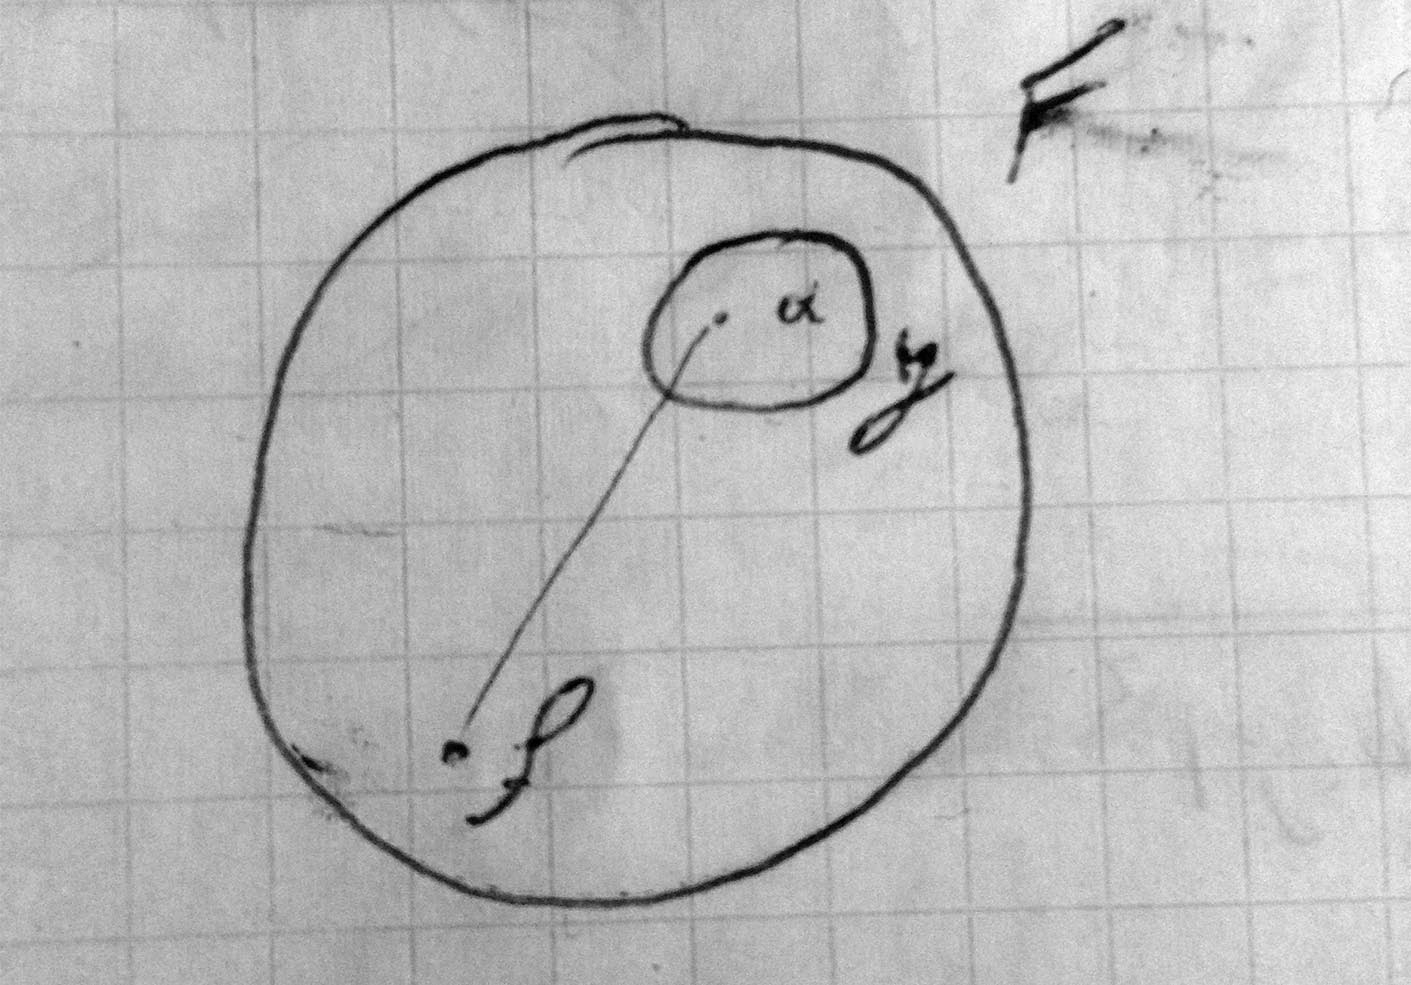
\includegraphics[width=0.5\textwidth]{Benaderingstheorie}
	\caption{Benaderingstheorie}
\end{figure}
$ F = C[-1,1] $ verzameling continue functies op -1,1 en $ y = P_4[-1,1]$ verzameling van veeltermen met graad 4 of minder op -1,1. f functie dat we willen benaderen.

\begin{exam}[Geef de definitie van een metrische, genormeerde, strikt genormeerde, unitaire en euclidische ruimte. Geef het verband tussen deze verschillende ruimten. Wat zijn de verbanden hiertussen?  Welke ruimte wordt C{[a,b]} met  de L2-afstand, de triviale afstand, de max-afstand. Bespreek het belang van deze ruimten in de benaderingstheorie]   

Aan de verzameling F een bepaalde structuur/eigenschappen opleggen. Hoe meer eigenschappen hoe meer dingen aantonen/analyseren:
\begin{description}
\item[Metrische ruimte $\rho(x,y)$] afstand meten tussen 2 punten. Beste benadering defini\"eren alsook de existentie / bestaans vraag.
\item[Genormeerde ruimte $||\vec{x}||$] defini\"eren we norm / grootte, spreken we van grootte van de fout. Alsook aantal benaderingen, de uniciteit (= zijn er 1 of meer oplossingen). 
\item[Unitaire ruimte $( \vec{x},\vec{y} ) $] ruimte met scalair product, loodrechte stand (orthogonaliteit) en strict genormeerd. Uitspraak over karakteristiek, weet je waar beste benadering ligt? Naarlaten van een loodlijn op de benaderingsruimte (de orthogonale projectie).
\item[Euclidische ruimte] is een unitaire ruimte met een eindige dimensie, je hebt een basis, je kan een punt kenmerken door een paar getallen. Algoritme / berekening.
\end{description}
\end{exam}

 \begin{figure}[h]
 \centering
\begin{tikzpicture}
\coordinate (O) at (0,0);
\foreach \j in {1,...,4} \draw (O) circle (5-\j);
\foreach \k/\text in {0/Metrische ruimte,1/Genormeerde ruimte,2/Unitaire ruimte,3/Euclidische ruite} \draw[decoration={text along path,reverse path,text align={align=center},text={\text}},decorate] (3.4-\k,0) arc (0:180:3.4-\k);
\begin{scope}[xshift=6cm]
\end{scope}
\end{tikzpicture}
  \caption{Onion ruimtes}
  \end{figure}

\section{Metrische ruimte $\rho(x,y)$}
Metriek / afstandsfunctie $\rho (x,y) $ met $ \rho : A x A \rightarrow \mathbb{R} $  
\begin{enumerate}
\item $\rho (x,y) \geq 0 $ positief 
\item $\rho (x,y) = 0 \Leftrightarrow x=y $ definiet
\item $\rho (x,y)=\rho(y,x) $ symmetrie
\item $\rho (x,y) \leq \rho(z,x)+\rho(z,y) $ driehoeksongelijkheid
\end{enumerate}
De eerste en derde kunnen afgeleid worden uit de anderen.

De afstand gedefinieerd als: $\rho(x,D) = \inf \left\{\rho(x,y)| y \in D\right\}$
Infimum omdat kleinste niet altijd bestat.

d is 'een' (er kan meer als 1 bestaan, bv cirkel) beste benadering in d voor x als: $\rho(x,d) = \rho(x,D) $. Een beste benadering bestaat niet altijd. 

\subsection{Voorbeelden}
\begin{description}
\item[Niet-klassieke]

\begin{description}
\item[Chordale afstand in $\mathbb{C}$]
De riemann bol, door de noordpool te verbinden met punt $z$, verkrijgt men een nieuw punt waar het de bol snijdt, de chordale afstand is de afstand tussen de nieuwe verkregen punten op de bol. \\
$\rho(0,noordpool) = \infty$ \\
$\rho(0,zuidpool) = oorsprong$ \\
$\rho(0,\infty) = 2$ \\
$\rho(0,1) = \sqrt{2}$ 
\item[Triviale afstand] Altijd 1 behalve als deze 0 moet zijn. Enkel in theorie gebruikt, om stellingen te ontkrachten. \\
$ \rho(x,y)=1 \,als\, x \neq y$ $\rho(0,\infty)=1 $\\ 
$ \rho(x,y)=0 \,als\, x=y$ $ \rho(0,0(0,1)) = 1 $
\item[Silvermanafstand] $\rho(A,B) = \#A \Delta B = \#(A \cup B) \setminus (A \cap B) $ Geeft de mate nabijheid van 2 groepen van studenten. 0 als groepen volledig overlappen.
\item[Hamming afstand] $\rho(0|0||,||00|)=2$
\item[Frobenius afstand] Geeft de mate van nabijheid tussen 2 matrixen weer. $\sqrt{\sum_i sum_j | a_{ij} - b_{ij}|^2}$

\begin{figure}[h]
	\centering
	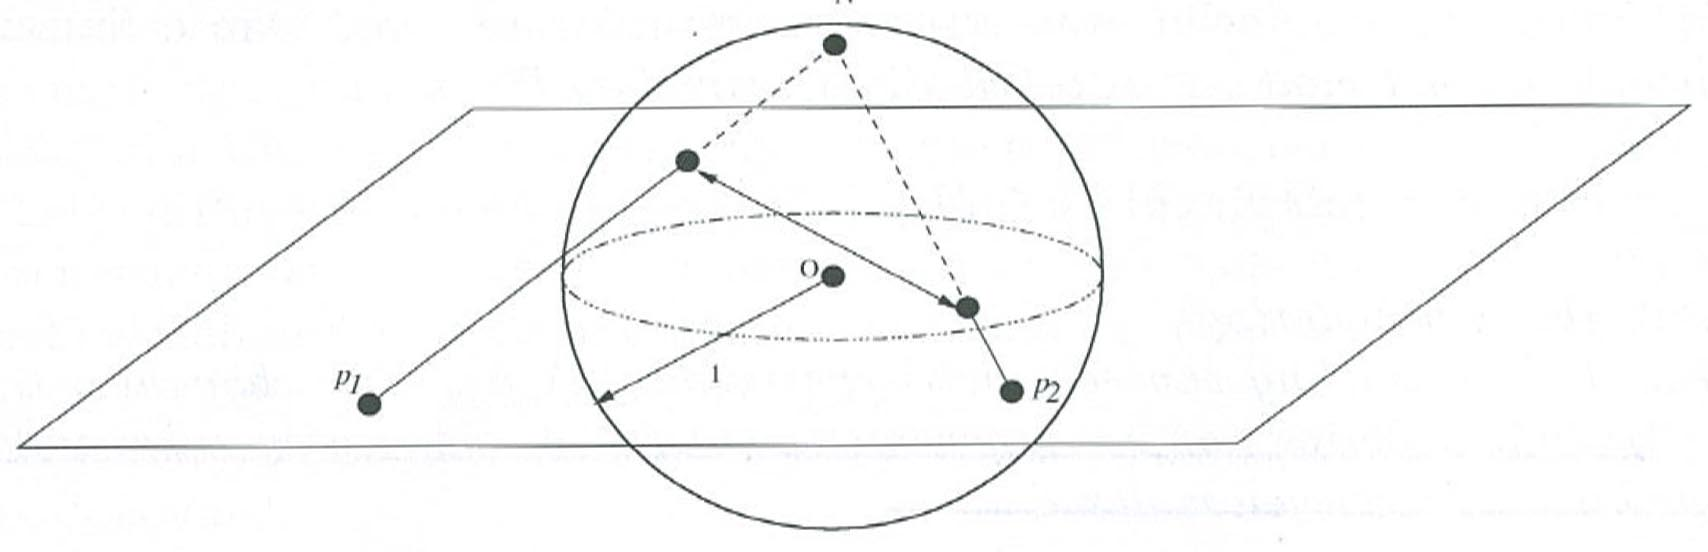
\includegraphics[width=0.5\textwidth]{ChordaleAfstand}
	\caption{Chordale afstand tussen punten $p_1$ en, $p_2$}
\end{figure}
\end{description}

\item[in continue functieruimten] $C[a,b]$
\begin{description}
\item[$L_\infty$-afstand] of max-afstand (gebruikt in minimax benadering): $\underset{x\in [a;b]}{\operatorname {max}}|f(x)-g(x)|=\rho(f,g) $\\
Check voorwaarden afstand: \\
$ f(x)-g(x)=f(x)-h(x)+h(x)-g(x)$ \\
$ |f(x)-g(x)| \leq|f(x)-h(x)|+ |h(x)-g(x)| $ \\
$\operatorname {max} |f(x)-g(x)| \leq \operatorname {max} |f(x)-h(x)|+ \operatorname {max} |h(x)-g(x)| $ \\
$\rho(f,g) \leq \rho(f,h)+\rho(h,g) $

\item[$L_p$ afstand] 
\begin{exam}$L_2[0, 1]$
$L_p[a,b]$ verzameling van functieklassen (functies die bijna overal gelijk zijn) die ook discontinue functies toelaat uitbreiding van $C[a,b]$. Verzameling van alle functies, waarvoor geldt dat $\sqrt[p]{\int_a^b w(x)|f(x)-g(x)|^p dx}$ aan alle voorwaarden voor een afstand voldoet, met $p \geq 1$ om aan laatste voorwaarde te voldoen. \\
$f=g \iff f(x)=g(x)$ b.o. (bijna overal of a.e. almost everywhere)
$\rho(f,g)=0$ en toch $f\neq g$. We maken geen onderscheid tussen functie $f$ en $g$ die bijna overal gelijk zijn. Wat is bijna overal? Dit is een term afkomstig uit de maattheorie, waarmee bedoeld wordt: overal behalve op een voor de theorie verwaarloosbaar deel, een verzameling van maat nul. Dit kan men zien als een lintje nemen van $\epsilon$ lengte, kunnen we dit verknippen en elk van deze punten bedekken? Bv rationele punten, dit is oneindig aftelbaar (men kan ze opsommen, oneindig veel) waardoor we steeds een kleiner stukje lint kunnen nemen $\frac{\epsilon}{2}$,$\frac{\epsilon}{4}$,$\frac{\epsilon}{8}$,\ldots\\ (We moeten integraal ook aanpassen van Rieman naar Libesque integraal.)
\textbf{$L_2$} kleinste kwadratenbenadering %TODO meer info? Examenvraag
\end{exam}
\end{description}
\item[in discrete functieruimten] 
\begin{description}
\item[Eindige dimensie] Aantal losse punten, $x_1,x_2,\ldots,x_n$ Verzameling van al discrete functies, vectoren van functiewaarden. $\mathbb{R}^N$ of $\mathbb{C}^N$, Vectoren van lengte N
\item[Oneindige dimensie] $l_p(\mathbb{R}), l_p(\mathbb{C})$ \\
$l_p = \sum_{i=1}^N w_i |f_i-g_i |^P < \infty $ \\
$l_\infty = \underset{i=1,\ldots,N}{\operatorname{max}} |f_i-g_i|$
\end{description} 
\end{description}

\section{Genormeerde ruimte $||\vec{x}||$}
\begin{enumerate}
\item $||\vec{x}|| \geq 0 $ positief definiete functionaal
\item $||\vec{x}|| = 0  \iff \vec{x} = \vec{0} $ positief definiete functionaal
\item $||a \vec{x}|| = |a| \cdot ||\vec{x}|| $ homogeniteitseigenschap
\item $||\vec{x}+\vec{y}|| \leq ||\vec{x}|| + ||\vec{y}|| $ driehoeksongelijkheid
\end{enumerate}
Door $\vec{y} = \vec{-x}$ bekomt men van 4de voorwaarde ook de 1ste voorwaarde. $||\vec{x}-\vec{x}|| \leq ||\vec{x}|| + ||\vec{-x}|| $ \\
$||0|| \leq ||\vec{x}|| + ||\vec{-x}|| $

\begin{enumerate}
\item Een genormeerde ruimte is ook metrisch \\
$||\vec{x}-\vec{y}||$ is een afstand $\rho(x,y)$
\item Zij $(a,\rho)$ een metrische vector ruimte dan is $\rho(\vec{0},\vec{x})$ een norm $\iff$
\begin{enumerate}
\item $\rho(\vec{x},\vec{y})=\rho(\vec{x}+\vec{z},\vec{y}+\vec{z)}$ translatie-invariantie
\item $\rho(a\vec{x},a\vec{y})=a\rho(\vec{x},\vec{y}) $ voor a $\in \mathbb{R}^+ (a \geq 0)$  homogeen
\end{enumerate}
\end{enumerate}
De triviale afstand is niet homogeen. $\rho(x,y) = 1, x \neq y$, $\rho(x,y) = 0, x = y$ Wordt niet 2 indien we $a \rho(x,y,)$ met $x \neq y$.



\begin{figure}[h]
	\centering
	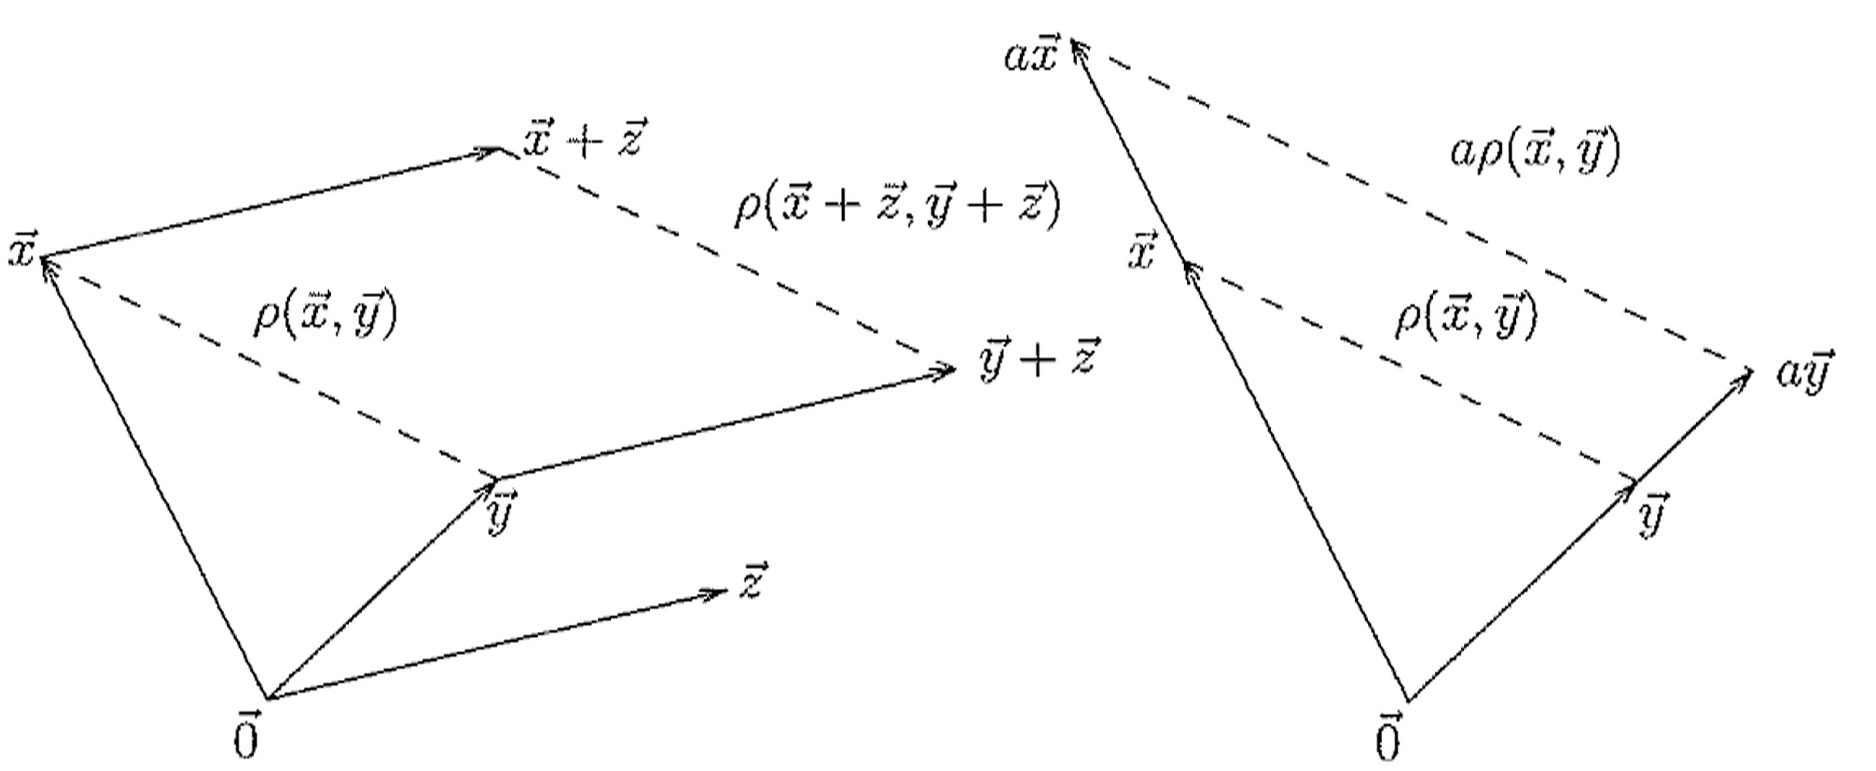
\includegraphics[width=0.5\textwidth]{TranslatieInvariantieHomogeniteitAfstandVectorruimte}
	\caption{Translatie-invariantie en homogeniteit van een afstand in een vectorruimte}
\end{figure}

\subsection{Voorbeelden}
\begin{description}
\item[B[a,b]] dit is de norm van de verzameling van continue functies op $[a,b]$ , $ \underset{x\in[a,b]}{\operatorname{sup}} |f(x)|$
$ |f(x)+g(x)| \leq |f(x)|+|g(x)| $ \\
$\operatorname {max}|f(x)+g(x)| \leq \operatorname {max}|f(x)|+ \operatorname {max} |g(x)| $
\item[$L_p$[a,b]] $\sqrt[p]{\int_a^b w(x)|f(x)|^p dx}=||f||_p$
\item[$\mathbb{R}^N,\mathbb{C}^N$] $\sqrt[p]{\sum_{i=1}^N w_i|f_i|^p dx}=||f||_p$
\end{description}

\subsection{Beste benadering}
$\tilde{B}(\vec{0},1)=\{(x,y)| \, ||(x,y)||=1\}$ of $\{\vec{x}| \, ||\vec{x}||=1\}$ \\
Al de punten liggen even ver naargelang de norm.
\begin{description}
\item [$l_2$] $\sqrt{x^2+y^2}=1$
\item[$l_1$] $|x|+|y|=1$
\item [$l_\infty$] $\operatorname{max}\{{|x|,|y|}\}=1$
\end{description}
\begin{figure}[h]
	\centering
	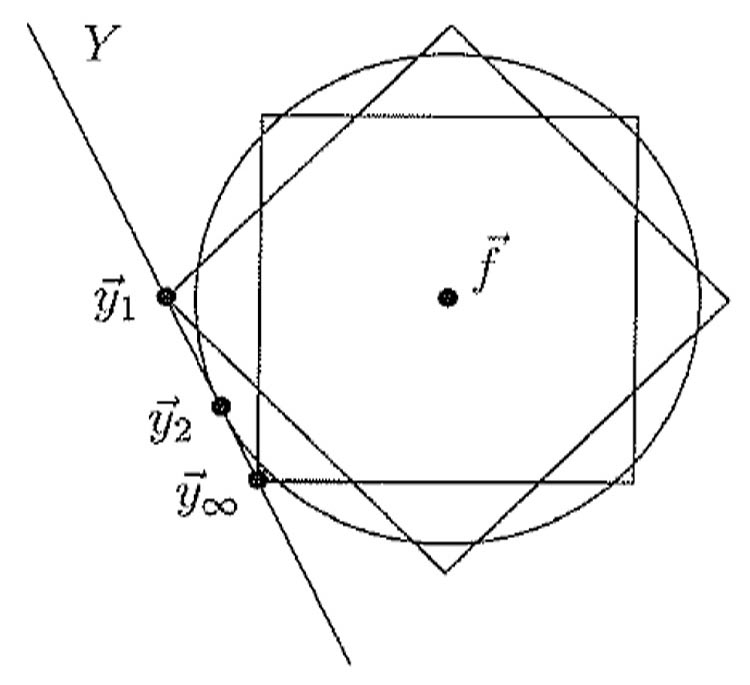
\includegraphics[width=0.5\textwidth]{BesteBenaderingPuntFVolgensNormen}
	\caption{Beste benadering voor het punt $\vec{f}$ volgens de 1-norm,2-norm,$\infty$-norm.}
\end{figure}
\begin{figure}[h]
	\centering
	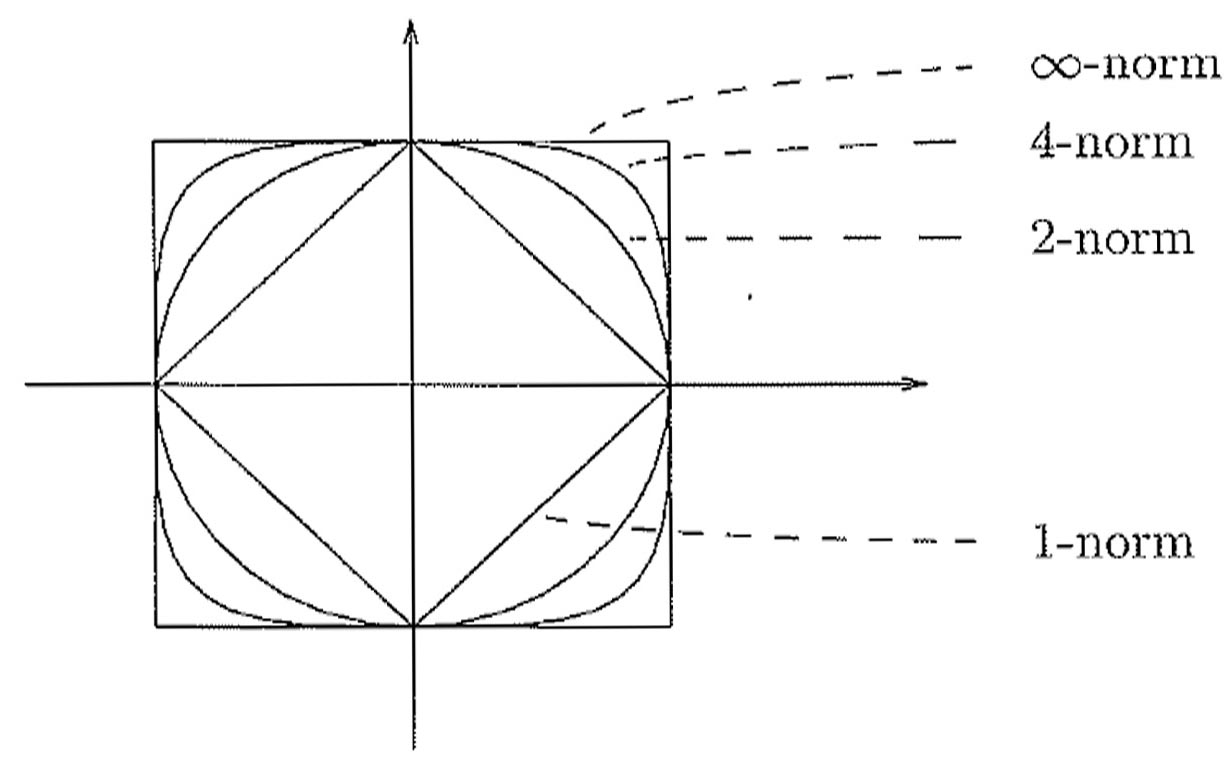
\includegraphics[width=0.5\textwidth]{EenheidscirkelsVlak}
	\caption{Eenheidscirkels in het vlak}
\end{figure}

Altijd maar 1 oplossing/punt als de bol strict convex is. Anders zou het kunnen zijn dat we oneindig veel oplossingen hebben.

\begin{figure}[h]
	\centering
	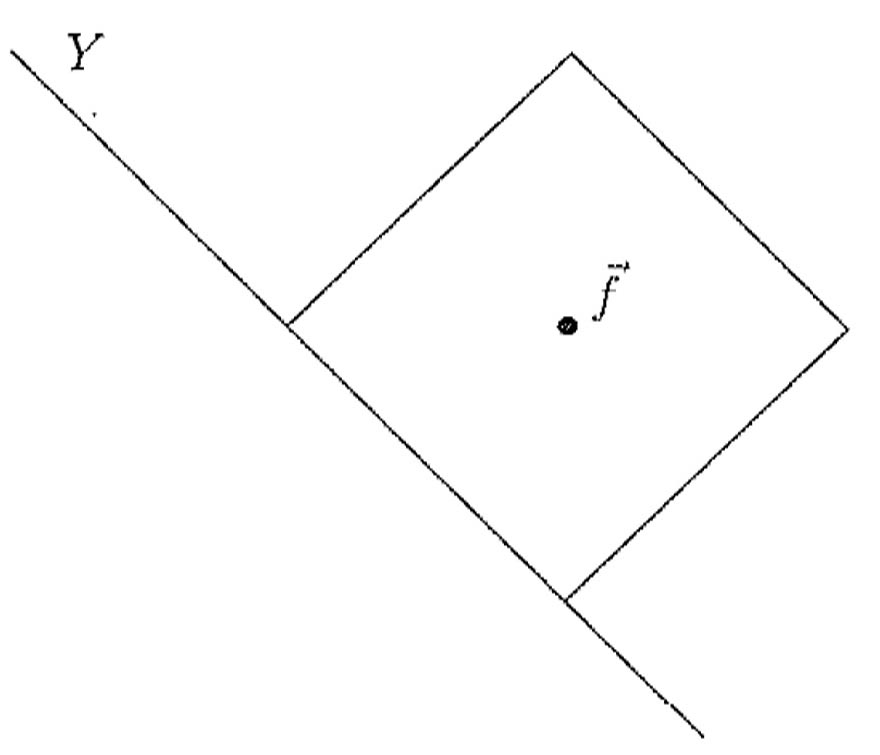
\includegraphics[width=0.5\textwidth]{MeervoudigheidBesteBenadering1Norm}
	\caption{Meervoudigheid van de beste benadering in de 1-norm}
\end{figure}

\subsection{Convexiteit} %TODO, wat aanvullen
\begin{exam} [Genormeerde ruimte, strikt genormeerde ruimte]
C is convex $\forall x_1,x_2 \in C: L(lijnstuk)(x_1,x_2) \in C $ \\
Waarom moet p steeds groter zijn als 1?
C is strict convex met $L(x_1,x_2)=\{\vec{x} | \vec{x} = \lambda \vec{x_1}+(1-\lambda) \vec{x_2} $ met $\lambda \in ((0,1) \}$ \\\\
$\vec{x_1},\vec{x_2} \in B(\vec{a},1)$ \\
$ ||\vec{a}-(\lambda\vec{x_1}+(1-\lambda)\vec{x_2})||=||\lambda\vec{a}-\lambda\vec{x_1}+(1-\lambda)\vec{a}-(1-\lambda)\vec{x_2}|| \leq |r|$ \\
$\lambda||\vec{a}-\vec{x_1}||+(1-\lambda)||\vec{a}-\vec{x_2}|| \leq r$ \\\\
$||\vec{x_1}|| = 1 = ||\vec{x_2}|| \rightarrow || \frac{x_1+x_2}{2} || <2 \rightarrow ||x_1+x_2||<2$
\end{exam}
\section{Unitaire ruimte $( \vec{x},\vec{y} ) $}
$(\cdot,\cdot):V*V \rightarrow \mathbb{R}$
\begin{enumerate}
\item $(a\vec{x},\vec{y})=a(\vec{x},\vec{y}$
\item $(\vec{x}+\vec{y}\vec{z})=(\vec{x},\vec{z})+(\vec{y},\vec{z})$
\item $(\vec{x},\vec{y})=(\vec{y},\vec{x})$ symmetrie
\item $(\vec{x},\vec{x}) > 0 \iff \vec{x} \neq \vec{0}$ definiet
\end{enumerate}
Aantal voorwaarden bij elkaar: $(\vec{x},a\vec{y})=\bar{a}(\vec{x},\vec{y})$

\subsection{Verband met vorige ruimte}
Cauchy-Schwarz $|(\vec{x},\vec{y})| \leq \sqrt{(\vec{x},\vec{x})}*\sqrt{(\vec{y},\vec{y})}$ \\
Te bewijzen: $\sqrt{(x+y,x+y)} \leq \sqrt{(x,x)}+\sqrt{(y,y)}$
\begin{enumerate}
\item Een unitaire ruimte is genormeerd $||\vec{x}||=\sqrt{(\vec{x},\vec{x})}$ is een norm.
\item Zij $(A,||\cdot||)$ een genormeerde ruimte dan geldt dat het unitair is als de norm voldoet aan de parallellogram gelijkheid. \\
\begin{form}
$ ||x+y||+||x-y||^2=2||x||^2+2||y||^2$ \\
$||\vec{x}|| = \sqrt{(\vec{x},\vec{x})}$
$(\vec{x},\vec{y})=1/4\{||x+y||^2-||x-y||^2\}$ is een scalair product.
\begin{figure}[h]
	\centering
	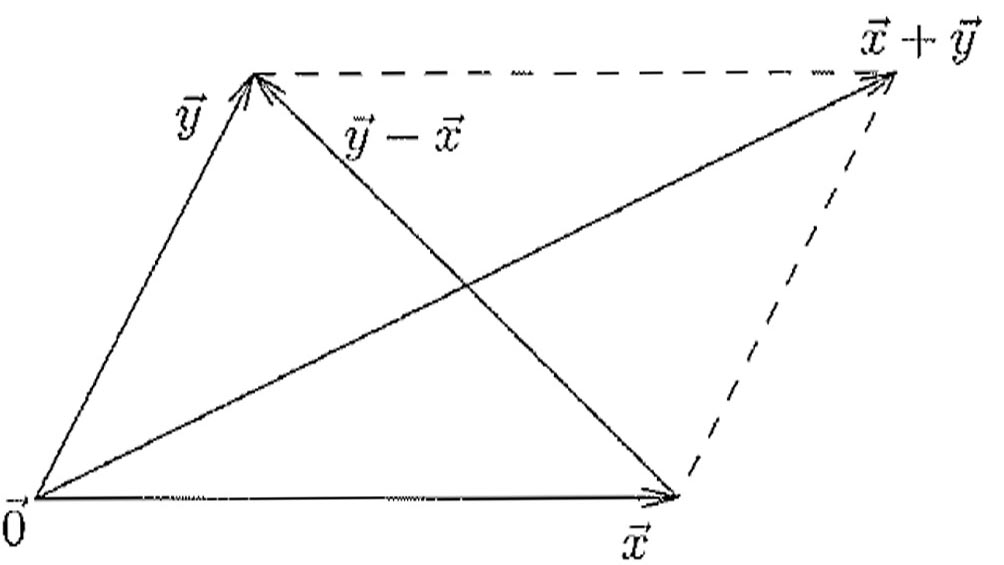
\includegraphics[width=0.5\textwidth]{ParallellogramgelijkheidVlak}
	\caption{Parallellogramgelijkheid in het vlak}
\end{figure}
\end{form}
\item Elke unitaire ruimte is strict genormeerd. Uniciteit is een unitaire ruimte. \\
$\left\{ \begin{array}{ll} ||\vec{x_1}||=||\vec{x_2}||=1\\ \vec{x_1} \neq \vec{x_2} \end{array} \right\} \rightarrow ||x_1 +x_2 || < 2$ \\
$|| x_1+x_2||^2 = 2||x_1||^2+2||x_2||^2-||x_1-x_2||^2 = 4- ||x_1-x_2||^2 \rightarrow ||x_1 +x_2 ||^2 < 4$ \\
Unitair $\rightarrow$ strikt genormeerd
\end{enumerate}
\subsection{Voorbeelden}
Ruimtes die overblijven: \\
\begin{description}
\item [$\mathbb{R}^N\, \mathbb{C}^N$ met $l_2$-norm]
$ (a\vec{x},y)=a(\vec{x},\vec{y}) $ \\
$(x,a\vec{y})=\overline{(a\vec{y},\vec{x})}=\bar{a}\overline{(y,x)}=\bar{a}(x,y)$ \\
$(x,y)=(\sum_{i=1}^n x_i \vec{e_i},\sum_{j=1}^n y_j \vec{e_j})=\sum_{i=1}^n\sum_{j=1}^n  x_i \vec{y_j}(\vec{e_i},\vec{e_j})=X^TG\bar{Y}$

Fundamentele metrische matrix: $G={\begin{vmatrix}\langle e_{1},e_{1}\rangle &\langle e_{1},e_{2}\rangle &\dots &\langle e_{1},e_{n}\rangle \\\langle e_{2},e_{1}\rangle &\langle e_{2},e_{2}\rangle &\dots &\langle e_{2},e_{n}\rangle \\\vdots &\vdots &\ddots &\vdots \\\langle e_{n},e_{1}\rangle &\langle e_{n},e_{2}\rangle &\dots &\langle e_{n},e_{n}\rangle \end{vmatrix}}$ \\

Controleren voor welke p aan de parallellogram gelijkheid voldoet:
2 vectoren (1,1) en (1,-1).
$ ||\vec{x} ||_p = \sqrt[p]{\sum |x_i|^p}$ \\
$ (x,y) = X^TG\bar{Y} $ \\
$\rho(\vec{x},\vec{y}) = \sqrt{(x-y)^TG(x-y)}$ klopt dit wel?  \\ %TODO
\begin{align*}
||x+y ||^2 + ||x-y||^2 &\stackrel{?}{=} 2 ||x||^2+2||y||^2  \\
||(2,0)||^2 + ||(0,2)||^2  &\stackrel{?}{=} 2 ||(1,1)||^2+2||(1,-1)||^2 \\
(\sqrt[p]{2^p+0^p})^2+(\sqrt[p]{0^p+2^p})^2 &\stackrel{?}{=} 2(\sqrt[p]{1^p+1^p})^2+2(\sqrt[p]{1^p+(-1)^p})^2 \\
4 + 4 &\stackrel{?}{=} 2*2^{2/p}+2*2^{2/p} \\
8 &\stackrel{?}{=} 4*2^{2/p} \\
2 &\stackrel{?}{=} 2^{2/p} \rightarrow p=2
\end{align*}
Alleen $p=2$ voldoet aan de parallellogram gelijkheid voldoet, aan al de andere is geen scalair product mee geassocieerd. 

\item [$L_p${[a,b]} met p=2 met $L_2$-norm] 


$(f,g)=\int_a^bw(x)f(x)\bar{g}(x) dx$ \\
$||f||_{L_2} = \sqrt{\int_a^b w(x) f^2(x) dx }$

\item[$l_2 (\mathbb{R}),l_2(\mathbb{C})$ met $l_2$-norm]
\end{description}
Ruimte die afvalt: 
\begin{description}
\item [C{[a,b]}, $max|f(x)|$] 


$f(x)=x$ op [0,1] \\
$g(x)=1$ op [0,1] \\
\begin{align*}
\operatorname{max}^|1+x|^2+\operatorname{max}|x-1|^2 &\neq 2\operatorname{max}|x|^2+2\operatorname{max}|1|^2 \\
2^2+1 &\neq 2+2
\end{align*}

\end{description}

\subsection{Orthogonaliteit}
\begin{enumerate}
\item $ \vec{x} \perp \vec{y}$ als $(\vec{x},\vec{y})=0$
\item $sin \perp cos$ als $(sin,cos)=0$ 
\item $sin \perp 1$
\item $x \perp D$ als $x\perp y$ met $y\in D$
\item Pythagoras als $\vec{x}\perp\vec{y} \rightarrow ||x+y||^2=||x||^2+||y||^2
$ \\
$ (x+y,x+y)=(x,x+y)+(y,(x+y)=(x,x)+(x,y)+(y,x)+(y,y)=(x,x)+(y,y) $
\end{enumerate}
Karakterisatie van beste benadering: Zij u een deelvectorruimte van een unitaire ruimte F en zij $y^* \in y$ zodat $f-y^* \perp y$ dan is $y*$ de beste beatnering voor f in y.
\begin{figure}[h]
	\centering
	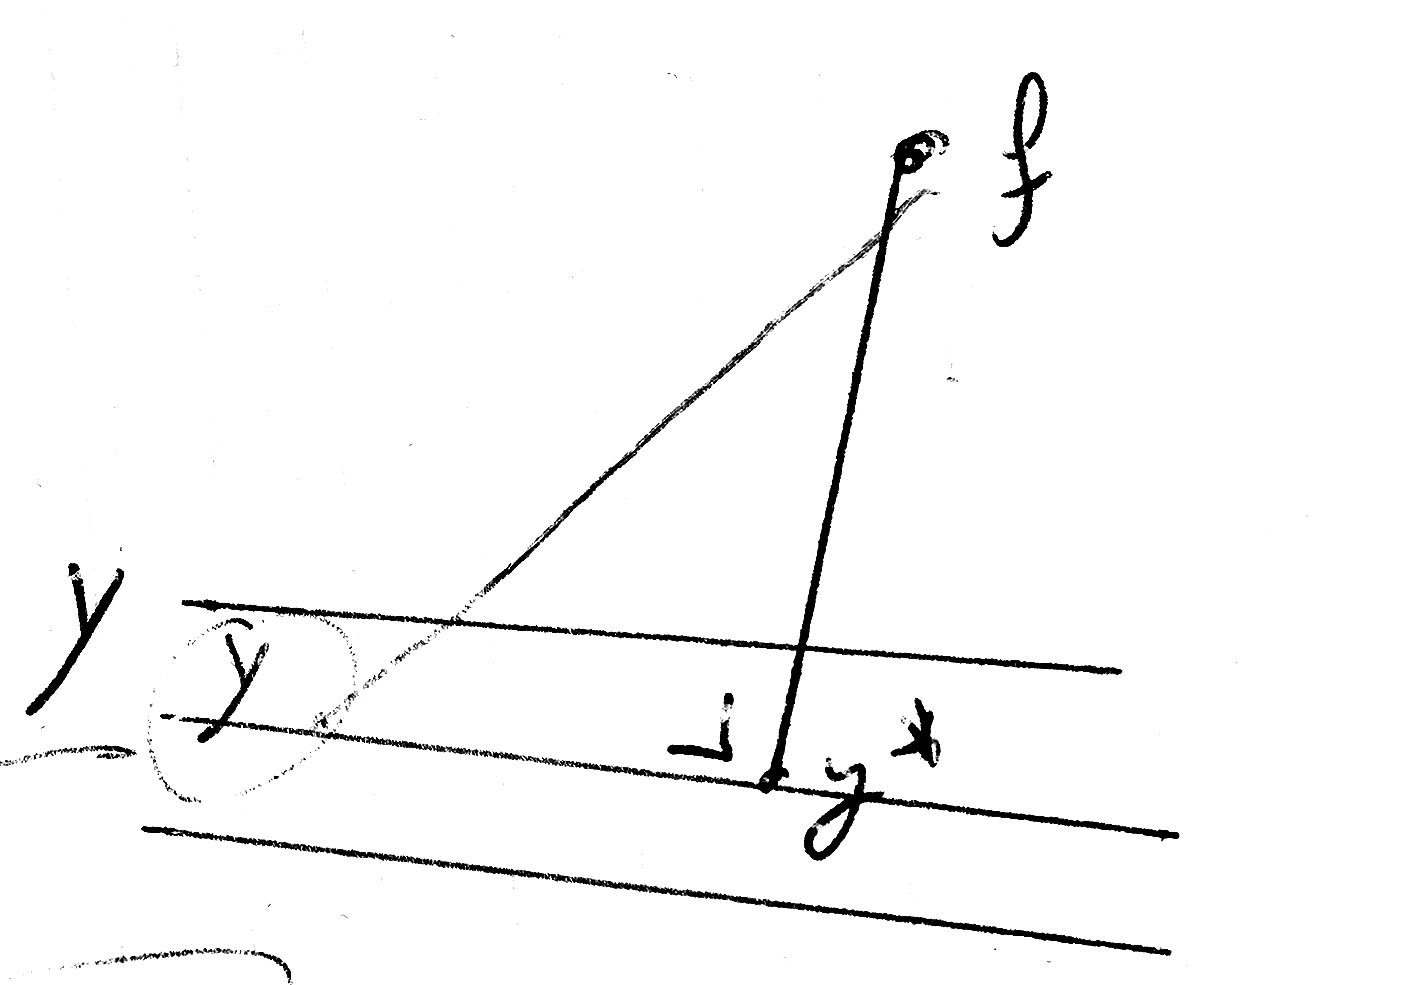
\includegraphics[width=0.5\textwidth]{LoodrechtY}
	\caption{Loodrecht}
\end{figure}
$ ||f-y||^2=||f-y^*||^2+||y-y^*||^2 $ \\
$ ||f-y||^2 \geq ||f-y^*||^2 $ \\
$ \rho(f,y) \geq \rho(f,y^*) $ \\



\section{Euclidische ruimte}
Euclidische ruimte = unitair + eindige dimensionaal, er bestaat een basis , elk element in de ruimte kunnen voorstellen door een aantal getallen (coordinaten).
\begin{figure}[h]
	\centering
	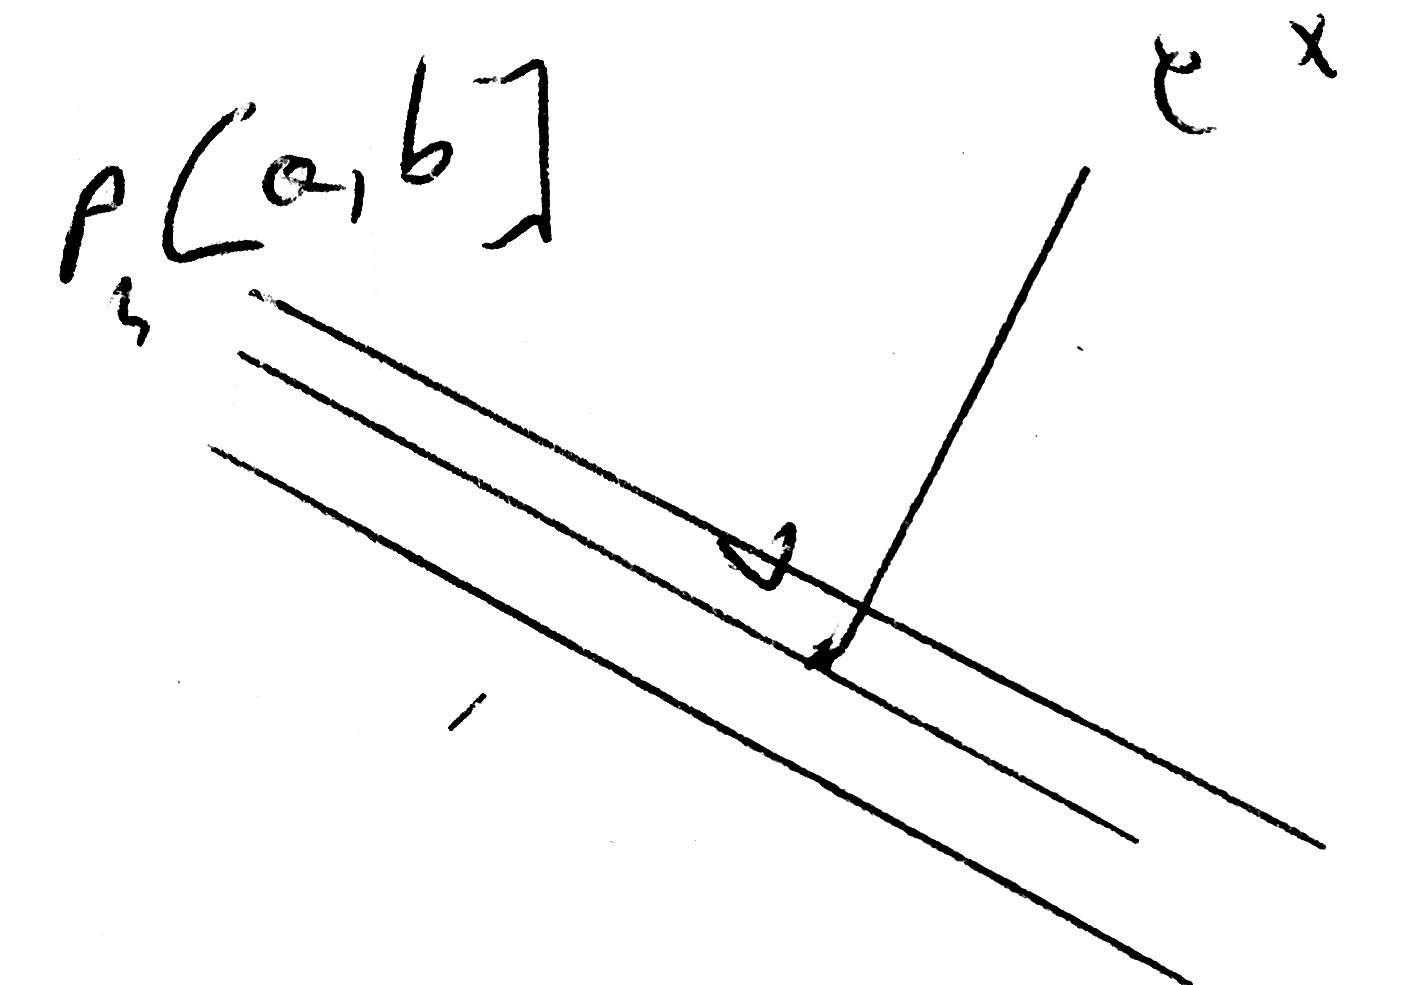
\includegraphics[width=0.5\textwidth]{EuclidischeRuimteLoodrecht2}
	\caption{$e^x$(uit oneindig dimensionale deelruimte) benaderen door een veelterm van graad 4 (5 dimensionale deelruimte)}
\end{figure}
Elke vector kan geschreven worden in de benaderingsruimte plus wat overschiet.
\begin{figure}[h]
	\centering
	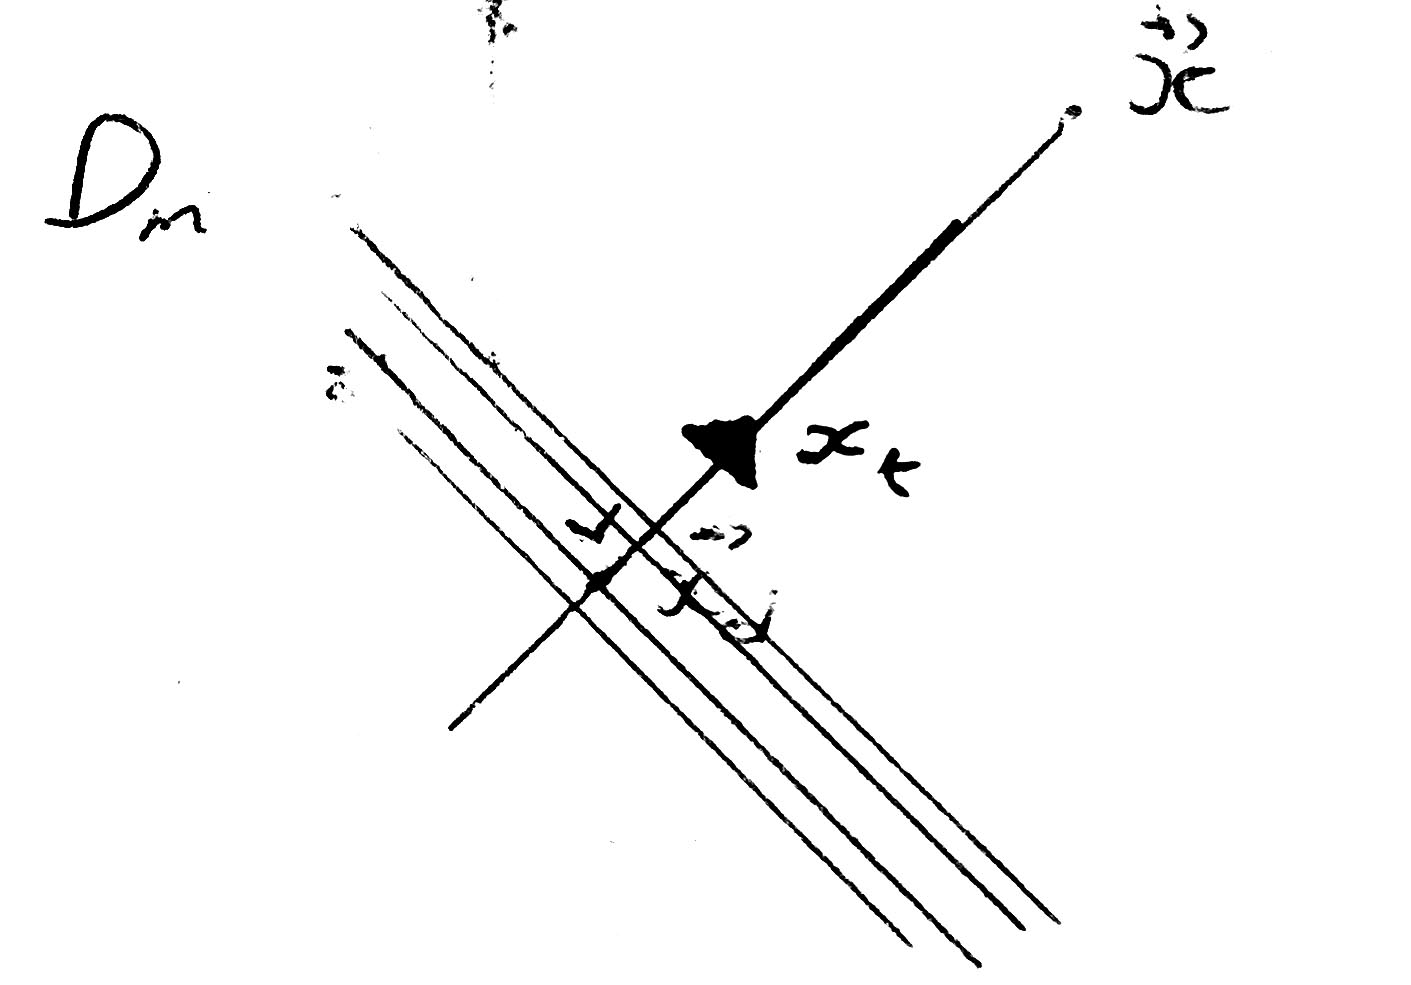
\includegraphics[width=0.5\textwidth]{EuclidischeRuimteLoodrecht}
	\caption{Euclidische ruimte loodrecht}
\end{figure}
$\vec{x}=\vec{x_d}+\vec{x_t}$ met $\vec{x_t}$ residu, benaderingsfout met $\vec{x_d} in D_m$ \\
$\vec{x_t} \perp D_m$ \\
$ \vec{x_d}=\sum_{k=0}^m a_k\vec{e_k} $ stel $\{\vec{e_1},\vec{e_2},\ldots\vec{e_m}\}$ en basis voor $D_m$
(tip: basis kan gaan van k gelijk aan 0 (jaar 2017) of 1 (jaar 2018), is enkel notatie)
Eis:
$\vec{x}-\vec{x_d}\perp \vec{e_i} \,\forall i$ \\
$(\vec{e_1},\vec{x}-\vec{x_d})=0$ $a_1(\vec{e_1},\vec{e_1})+a_2(\vec{e_2},\vec{e_1})+\ldots+a_m(\vec{e_m},\vec{e_1}) = (x,\vec{e_1}) = \sum_{k=1}^m a_k(\vec{e_1},\vec{e_k})=(\vec{e_1},x)$ \\ 
$(\vec{e_2},\vec{x}-\vec{x_d})=0$ $ \sum_{k=1}^m a_k(\vec{e_2},\vec{e_k})=(\vec{e_2},x)$ \\
\vdots \\
$(\vec{e_m},\vec{x}-\vec{x_d})=0$ $ \sum_{k=1}^m a_k(\vec{e_m},\vec{e_k})=(\vec{e_m},x)$ \\
$Ga=b$ (normaalstelsel) met G gramiaanmatrix \\
${\begin{bmatrix}\langle e_{1},e_{1}\rangle &\langle e_{1},e_{2}\rangle &\dots &\langle e_{1},e_{n}\rangle \\\langle e_{2},e_{1}\rangle &\langle e_{2},e_{2}\rangle &\dots &\langle e_{2},e_{n}\rangle \\\vdots &\vdots &\ddots &\vdots \\\langle e_{n},e_{1}\rangle &\langle e_{n},e_{2}\rangle &\dots &\langle e_{n},e_{n}\rangle \end{bmatrix}} * \begin{bmatrix} a_1 \\ a_2 \\ \vdots \\ a_n \end{bmatrix} = \begin{bmatrix} (x,e_1) \\ (x,e_2) \\ \vdots \\ (x,e_n)    \end{bmatrix}  $ \\

Gramiaanmatrix is symmetrisch positief definiet, als re\"el scalair product dat hermetisch positief definiet. \\
Symmetrisch: alleen maar positieve eigenwaarden.
$V^TGV=|| v_1 \vec{x_1} + v_2\vec{x_2} + \ldots +v_m \vec{x_m}||^2$ \\
Positief: $V^TGV > 0$ als $V\neq 0$ \\
Definiet: $V^TGV=0$ als $V=0$ Betekent dat de matrix altijd inverteerbaar is (een reguliere matrix), alle eigenwaarden zijn strict positief. Stelsel altijd een oplossing heeft. Oplossing altijd uniek.
\begin{figure}[h]
	\centering
	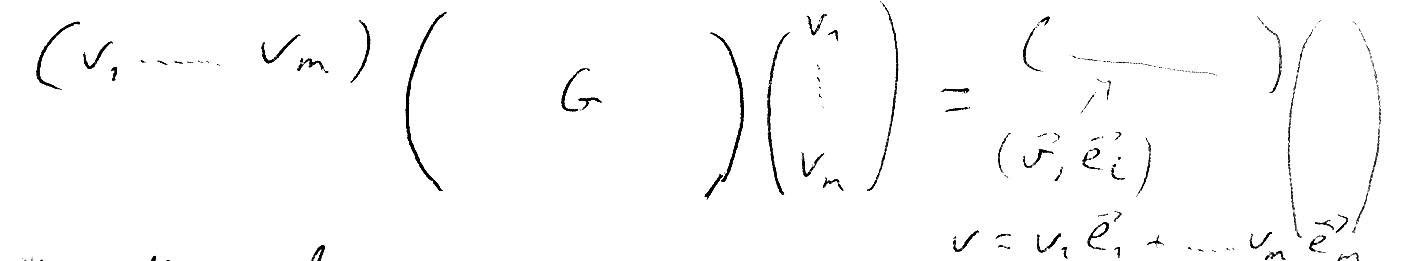
\includegraphics[width=0.5\textwidth]{SPDMatrix}
	\caption{SPD Matrix}
\end{figure}

\subsection{Orthogonale vectoren}
\begin{equation*}
\vec{e_i} \perp \vec{e_j} \, i\neq j
\end{equation*}
\begin{equation*}
a_k = \frac{(\vec{e_k},\vec{x})}{(\vec{e_k},\vec{e_k})} 
\end{equation*}
\begin{equation*}
\vec{x} \approx \vec{x_d} = \sum_{k=1}^m \frac{(\vec{e_k},\vec{x})}{(\vec{e_k},\vec{e_k})}\vec{e_k}
\end{equation*}

Benader $e^x$ in $P_4[-1,1]$
\begin{equation*}
(f,g)=\int_{-1}^1 f.g dx
\end{equation*}
\begin{equation*}
y_4(x)=a_0+a_1x+a_2x^2+a_3x^3+a_4x^4
\end{equation*}
\begin{equation*}
{\begin{bmatrix}\langle 1,1\rangle &\langle x,1 \rangle &\dots &\langle x^4,1\rangle \\\langle 1,x\rangle &\langle x,x \rangle &\dots &\langle x^4,x\rangle \\\vdots &\vdots &\ddots &\vdots \\\langle 1,x^4\rangle &\langle x^2,x^4\rangle &\dots &\langle x^4,x^4 \rangle \end{bmatrix}} * \begin{bmatrix} a_1 \\ a_2 \\ \vdots \\ a_n \end{bmatrix} = \begin{bmatrix} (e^x,1) \\ (e^x,x) \\ \vdots \\ (e^x,x^4)    \end{bmatrix}  
\end{equation*}

\subsection{Gram-Schmidt}
Opstellen van een orthogonale basis. \\
Vertrekt van een schuine basis $\vec{x_1},\vec{x_2},\ldots,\vec{x_m} \rightarrow \vec{y_1},\vec{y_2},\ldots,\vec{y_m}$ orthogonale basis.
\begin{equation*}
\vec{x_1}:\vec{y_1} = \vec{x_1}\lambda_1 \text{ normalisatie}
\end{equation*}
\begin{equation*}
\vec{x_2}:\vec{y_2}=\lambda_2(\vec{x_2}-a_1\vec{y_1}) \text{ met } (\vec{y_2},\vec{y_1})=0
\end{equation*}
\begin{equation*}
a_1 = \frac{(\vec{x_2},\vec{y_1})}{(,\vec{y_1},\vec{y_1})}
\end{equation*}
3 vergelijkingen waar je de 3 getallen kunt halen.
\begin{equation*}
x_i : \vec{y_i} = \lambda (\vec{x_i}-a_1\vec{y_1}\ldots a_{i-1}\vec{y_{i-1}})
\end{equation*}
\begin{equation*}
\rightarrow a_1 = \frac{(\vec{x_i},\vec{y_1})}{(\vec{y_1},\vec{y_1})}
\end{equation*}
\begin{equation*}
\rightarrow a_2 = \frac{(\vec{x_i},\vec{y_2})}{(\vec{y_2},\vec{y_2})}
\end{equation*}
\begin{equation*}
\vec{y_2} \perp \vec{y_1}
\end{equation*}
\begin{equation*}
\vec{y_i} \perp \vec{y_{i-1}}
\end{equation*}
Waar $ || y_2||= ( \vec{y_2},\vec{y_2})=1 $ en $ (\vec{y_i},\vec{y_{i-1}})=0$

\subsubsection{Voorbeeld}
$P_4[-1,1]$ met $(f,q)=\int_{-1}^1 f(x)g(x)dx$ $(L_2)$ \\
$1,x,x^2,x^3,x^4 \rightarrow P_0(x),P_1(x),\ldots,P_4(x)$ \\\\
$1.P_0(x)=\lambda_0.1$ eis $(P_0,P_0)=1$ \\
$\int_{-1}^1\lambda_0^2dx = 1 \rightarrow [\lambda_0^2*x]_{-1}^1 \rightarrow 2\lambda_0^2=1 \rightarrow \lambda_0=\frac{1}{\sqrt{2}}$ \\
$ P_0(x) = \frac{1}{\sqrt{2}}$ \\\\
$x: P_1(x)=\lambda_1(x-a_0P_0(x))$ \\
$a_0=\frac{(x,P_0)}{(P_0,P_0)} = \int_{-1}^1 x \frac{1}{\sqrt{2}} dx = [\frac{x^2}{2 \sqrt{2}}]_{-1}^1=0$\\
$P_1=\lambda_1 x$ \\
Eis $(P_1,P_0)= 0$ \\
$\int \frac{1}{\sqrt{2}}\lambda_1 x dx =0$ \\
Eis$(P_1,P_1)= 1$ \\
$\int \lambda_1x\lambda_1x=1 \rightarrow \int \lambda_1^2 x^2 dx = 1$ \\
$\frac{2\lambda_1^2}{3}=1 \rightarrow \lambda_1 = \sqrt{\frac{3}{2}}$ \\\\
Voor $P_2$ en verder zie boek p34

Voorbeeld: \\
$e^x \approx y_4(x)=a_0+a_1x+\ldots+a_4x^4$ \\
$ = b_0P_0(x)+b_1P_1(x)+\ldots+b_4P_4(x)$\\
\begin{equation*}
b_k = \frac{\int_{-1}^1 e^xP_k(x) dx}{\int_{-1}^1 P_k^2(x) dx}
\end{equation*}